\documentclass[border=8pt]{standalone}
\usepackage{fontspec}
\setmainfont{Carlito}
\setsansfont{Carlito}
\usepackage{tikz}
\usetikzlibrary{positioning, calc}

\definecolor{meetgreen}{RGB}{80,160,100}
\definecolor{partamber}{RGB}{210,170,60}
\definecolor{failred}{RGB}{200,90,80}
\definecolor{rowgrey}{RGB}{248,248,250}
\definecolor{headblue}{RGB}{70,130,180}
\definecolor{neutralgrey}{RGB}{100,100,110}
\definecolor{highlightgreen}{RGB}{238,250,238}
\definecolor{linegrey}{RGB}{220,220,225}

\begin{document}
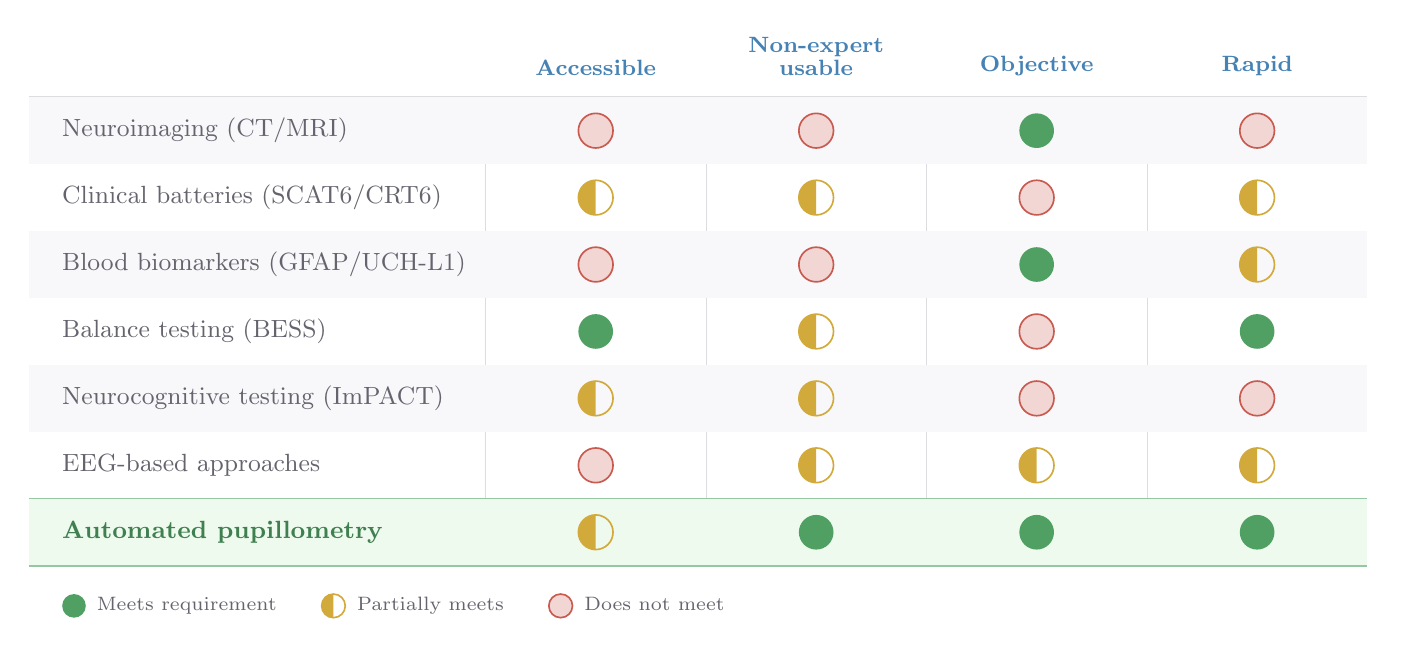
\begin{tikzpicture}[every node/.style={font=\sffamily}]

% Grid dimensions
\def\colw{2.8cm}
\def\rowh{0.85cm}
\def\labelw{5.8cm}
\def\totalw{\labelw + 4*\colw}
\def\circr{0.22cm}

% Column headers
\node[anchor=south, font=\footnotesize\bfseries, text=headblue, align=center, text width=\colw]
  at (\labelw + 0.5*\colw, 0.15) {Accessible};
\node[anchor=south, font=\footnotesize\bfseries, text=headblue, align=center, text width=\colw]
  at (\labelw + 1.5*\colw, 0.15) {Non-expert\\[-1pt]usable};
\node[anchor=south, font=\footnotesize\bfseries, text=headblue, align=center, text width=\colw]
  at (\labelw + 2.5*\colw, 0.15) {Objective};
\node[anchor=south, font=\footnotesize\bfseries, text=headblue, align=center, text width=\colw]
  at (\labelw + 3.5*\colw, 0.15) {Rapid};

% Header line
\draw[linegrey, thick] (0,0) -- (17.0,0);

% Vertical column separators (thin)
\foreach \i in {0,1,2,3} {
  \draw[linegrey, very thin] (\labelw + \i*\colw, 0) -- (\labelw + \i*\colw, -6*\rowh);
}

% === Helper: filled circle (green) ===
% === Helper: half circle (amber) ===
% === Helper: empty circle (red) ===

% Row 1: Neuroimaging (shaded)
\fill[rowgrey] (0, -\rowh) rectangle (17.0, 0);
\node[anchor=west, font=\small, text=neutralgrey] at (0.3, -0.5*\rowh) {Neuroimaging (CT/MRI)};
\fill[failred!25] (\labelw + 0.5*\colw, -0.5*\rowh) circle (\circr);
\draw[failred, semithick] (\labelw + 0.5*\colw, -0.5*\rowh) circle (\circr);
\fill[failred!25] (\labelw + 1.5*\colw, -0.5*\rowh) circle (\circr);
\draw[failred, semithick] (\labelw + 1.5*\colw, -0.5*\rowh) circle (\circr);
\fill[meetgreen] (\labelw + 2.5*\colw, -0.5*\rowh) circle (\circr);
\fill[failred!25] (\labelw + 3.5*\colw, -0.5*\rowh) circle (\circr);
\draw[failred, semithick] (\labelw + 3.5*\colw, -0.5*\rowh) circle (\circr);

% Row 2: Clinical batteries
\node[anchor=west, font=\small, text=neutralgrey] at (0.3, -1.5*\rowh) {Clinical batteries (SCAT6/CRT6)};
% Half circles for amber
\begin{scope}
  \clip (\labelw + 0.5*\colw - \circr, -1.5*\rowh - \circr) rectangle (\labelw + 0.5*\colw, -1.5*\rowh + \circr);
  \fill[partamber] (\labelw + 0.5*\colw, -1.5*\rowh) circle (\circr);
\end{scope}
\draw[partamber, semithick] (\labelw + 0.5*\colw, -1.5*\rowh) circle (\circr);

\begin{scope}
  \clip (\labelw + 1.5*\colw - \circr, -1.5*\rowh - \circr) rectangle (\labelw + 1.5*\colw, -1.5*\rowh + \circr);
  \fill[partamber] (\labelw + 1.5*\colw, -1.5*\rowh) circle (\circr);
\end{scope}
\draw[partamber, semithick] (\labelw + 1.5*\colw, -1.5*\rowh) circle (\circr);

\fill[failred!25] (\labelw + 2.5*\colw, -1.5*\rowh) circle (\circr);
\draw[failred, semithick] (\labelw + 2.5*\colw, -1.5*\rowh) circle (\circr);

\begin{scope}
  \clip (\labelw + 3.5*\colw - \circr, -1.5*\rowh - \circr) rectangle (\labelw + 3.5*\colw, -1.5*\rowh + \circr);
  \fill[partamber] (\labelw + 3.5*\colw, -1.5*\rowh) circle (\circr);
\end{scope}
\draw[partamber, semithick] (\labelw + 3.5*\colw, -1.5*\rowh) circle (\circr);

% Row 3: Blood biomarkers (shaded)
\fill[rowgrey] (0, -3*\rowh) rectangle (17.0, -2*\rowh);
\node[anchor=west, font=\small, text=neutralgrey] at (0.3, -2.5*\rowh) {Blood biomarkers (GFAP/UCH-L1)};
\fill[failred!25] (\labelw + 0.5*\colw, -2.5*\rowh) circle (\circr);
\draw[failred, semithick] (\labelw + 0.5*\colw, -2.5*\rowh) circle (\circr);
\fill[failred!25] (\labelw + 1.5*\colw, -2.5*\rowh) circle (\circr);
\draw[failred, semithick] (\labelw + 1.5*\colw, -2.5*\rowh) circle (\circr);
\fill[meetgreen] (\labelw + 2.5*\colw, -2.5*\rowh) circle (\circr);
\begin{scope}
  \clip (\labelw + 3.5*\colw - \circr, -2.5*\rowh - \circr) rectangle (\labelw + 3.5*\colw, -2.5*\rowh + \circr);
  \fill[partamber] (\labelw + 3.5*\colw, -2.5*\rowh) circle (\circr);
\end{scope}
\draw[partamber, semithick] (\labelw + 3.5*\colw, -2.5*\rowh) circle (\circr);

% Row 4: Balance testing
\node[anchor=west, font=\small, text=neutralgrey] at (0.3, -3.5*\rowh) {Balance testing (BESS)};
\fill[meetgreen] (\labelw + 0.5*\colw, -3.5*\rowh) circle (\circr);
\begin{scope}
  \clip (\labelw + 1.5*\colw - \circr, -3.5*\rowh - \circr) rectangle (\labelw + 1.5*\colw, -3.5*\rowh + \circr);
  \fill[partamber] (\labelw + 1.5*\colw, -3.5*\rowh) circle (\circr);
\end{scope}
\draw[partamber, semithick] (\labelw + 1.5*\colw, -3.5*\rowh) circle (\circr);
\fill[failred!25] (\labelw + 2.5*\colw, -3.5*\rowh) circle (\circr);
\draw[failred, semithick] (\labelw + 2.5*\colw, -3.5*\rowh) circle (\circr);
\fill[meetgreen] (\labelw + 3.5*\colw, -3.5*\rowh) circle (\circr);

% Row 5: Neurocognitive (shaded)
\fill[rowgrey] (0, -5*\rowh) rectangle (17.0, -4*\rowh);
\node[anchor=west, font=\small, text=neutralgrey] at (0.3, -4.5*\rowh) {Neurocognitive testing (ImPACT)};
\begin{scope}
  \clip (\labelw + 0.5*\colw - \circr, -4.5*\rowh - \circr) rectangle (\labelw + 0.5*\colw, -4.5*\rowh + \circr);
  \fill[partamber] (\labelw + 0.5*\colw, -4.5*\rowh) circle (\circr);
\end{scope}
\draw[partamber, semithick] (\labelw + 0.5*\colw, -4.5*\rowh) circle (\circr);
\begin{scope}
  \clip (\labelw + 1.5*\colw - \circr, -4.5*\rowh - \circr) rectangle (\labelw + 1.5*\colw, -4.5*\rowh + \circr);
  \fill[partamber] (\labelw + 1.5*\colw, -4.5*\rowh) circle (\circr);
\end{scope}
\draw[partamber, semithick] (\labelw + 1.5*\colw, -4.5*\rowh) circle (\circr);
\fill[failred!25] (\labelw + 2.5*\colw, -4.5*\rowh) circle (\circr);
\draw[failred, semithick] (\labelw + 2.5*\colw, -4.5*\rowh) circle (\circr);
\fill[failred!25] (\labelw + 3.5*\colw, -4.5*\rowh) circle (\circr);
\draw[failred, semithick] (\labelw + 3.5*\colw, -4.5*\rowh) circle (\circr);

% Row 6: EEG
\node[anchor=west, font=\small, text=neutralgrey] at (0.3, -5.5*\rowh) {EEG-based approaches};
\fill[failred!25] (\labelw + 0.5*\colw, -5.5*\rowh) circle (\circr);
\draw[failred, semithick] (\labelw + 0.5*\colw, -5.5*\rowh) circle (\circr);
\begin{scope}
  \clip (\labelw + 1.5*\colw - \circr, -5.5*\rowh - \circr) rectangle (\labelw + 1.5*\colw, -5.5*\rowh + \circr);
  \fill[partamber] (\labelw + 1.5*\colw, -5.5*\rowh) circle (\circr);
\end{scope}
\draw[partamber, semithick] (\labelw + 1.5*\colw, -5.5*\rowh) circle (\circr);
\begin{scope}
  \clip (\labelw + 2.5*\colw - \circr, -5.5*\rowh - \circr) rectangle (\labelw + 2.5*\colw, -5.5*\rowh + \circr);
  \fill[partamber] (\labelw + 2.5*\colw, -5.5*\rowh) circle (\circr);
\end{scope}
\draw[partamber, semithick] (\labelw + 2.5*\colw, -5.5*\rowh) circle (\circr);
\begin{scope}
  \clip (\labelw + 3.5*\colw - \circr, -5.5*\rowh - \circr) rectangle (\labelw + 3.5*\colw, -5.5*\rowh + \circr);
  \fill[partamber] (\labelw + 3.5*\colw, -5.5*\rowh) circle (\circr);
\end{scope}
\draw[partamber, semithick] (\labelw + 3.5*\colw, -5.5*\rowh) circle (\circr);

% Separator before pupillometry
\draw[meetgreen!60, thick] (0, -6*\rowh) -- (17.0, -6*\rowh);

% Row 7: Automated pupillometry (highlighted)
\fill[highlightgreen] (0, -7*\rowh) rectangle (17.0, -6*\rowh);
\node[anchor=west, font=\small\bfseries, text=meetgreen!80!black] at (0.3, -6.5*\rowh) {Automated pupillometry};
\begin{scope}
  \clip (\labelw + 0.5*\colw - \circr, -6.5*\rowh - \circr) rectangle (\labelw + 0.5*\colw, -6.5*\rowh + \circr);
  \fill[partamber] (\labelw + 0.5*\colw, -6.5*\rowh) circle (\circr);
\end{scope}
\draw[partamber, semithick] (\labelw + 0.5*\colw, -6.5*\rowh) circle (\circr);
\fill[meetgreen] (\labelw + 1.5*\colw, -6.5*\rowh) circle (\circr);
\fill[meetgreen] (\labelw + 2.5*\colw, -6.5*\rowh) circle (\circr);
\fill[meetgreen] (\labelw + 3.5*\colw, -6.5*\rowh) circle (\circr);

% Bottom line
\draw[meetgreen!60, thick] (0, -7*\rowh) -- (17.0, -7*\rowh);

% Legend
\node[anchor=west, font=\scriptsize, text=neutralgrey] at (0.3, -7.6*\rowh) {%
  \tikz[baseline=-0.5ex]{\fill[meetgreen] (0,0) circle (0.15cm);}\enspace Meets requirement\qquad
  \tikz[baseline=-0.5ex]{\begin{scope}\clip (-0.15,-.15) rectangle (0,0.15); \fill[partamber] (0,0) circle (0.15cm);\end{scope}\draw[partamber,semithick] (0,0) circle (0.15cm);}\enspace Partially meets\qquad
  \tikz[baseline=-0.5ex]{\fill[failred!25] (0,0) circle (0.15cm); \draw[failred,semithick] (0,0) circle (0.15cm);}\enspace Does not meet};

\end{tikzpicture}
\end{document}
